
\section*{Task 4}
    In this case we need to convert a 4-bit number into its complement 
    to two. A truth table is built first with four outputs corresponding 
    to the four input bits of the number complemented, as shown below.
    \begin{table}[H]
        \begin{center}
        \begin{tabular}{|c|c|c|c||c|c|c|c|}
        \hline
        \multicolumn{4}{|c||}{4-Bit In} & \multicolumn{4}{|c|}{2-Comp. Out}
        \\ \hline
        $d$ & $c$ & $b$ & $a$ & $f_{d}$ & $f_{c}$ & $f_{b}$ & $f_{a}$\\
        \hline \hline
        0 & 0 & 0 & 0 & 0 & 0 & 0 & 0\\ \hline
        0 & 0 & 0 & 1 & 1 & 1 & 1 & 1\\ \hline
        0 & 0 & 1 & 0 & 1 & 1 & 1 & 0\\ \hline
        0 & 0 & 1 & 1 & 1 & 1 & 0 & 1\\ \hline
        0 & 1 & 0 & 0 & 1 & 1 & 0 & 0\\ \hline
        0 & 1 & 0 & 1 & 1 & 0 & 1 & 1\\ \hline
        0 & 1 & 1 & 0 & 1 & 0 & 1 & 0\\ \hline
        0 & 1 & 1 & 1 & 1 & 0 & 0 & 1\\ \hline
        1 & 0 & 0 & 0 & 1 & 0 & 0 & 0\\ \hline
        1 & 0 & 0 & 1 & 0 & 1 & 1 & 1\\ \hline
        1 & 0 & 1 & 0 & 0 & 1 & 1 & 0\\ \hline
        1 & 0 & 1 & 1 & 0 & 1 & 0 & 1\\ \hline
        1 & 1 & 0 & 0 & 0 & 1 & 0 & 0\\ \hline
        1 & 1 & 0 & 1 & 0 & 0 & 1 & 1\\ \hline
        1 & 1 & 1 & 0 & 0 & 0 & 1 & 0\\ \hline
        1 & 1 & 1 & 1 & 0 & 0 & 0 & 1\\ \hline
        \end{tabular}
        \caption{Outputs with complement to two.}
        \end{center}
        \end{table}
        \par
        The output functions are expressed based on the minternms.
        They are simplified using Karnaugh's Maps. Starting with $f_d$ function:\par
        \[
            f_{d}=\sum{(m_1,m_2,m_3,m_4,m_5,m_6,m_7,m_8)}
        \]
        \begin{centering}
            \begin{Karnaugh}
                \minterms{1,2,3,4,5,6,7,8}
                \maxterms{0,9,10,11,12,13,14,15}
                \implicantsol{8}{red}
                \implicant{4}{6}{red}
                \implicant{1}{3}{red}
                \implicant{2}{6}{blue}
            \end{Karnaugh}
        \par\end{centering}
        Solving the map with the indicated groups, the simplified 
        function remains as:
        \[
            \boxed{f_{d}=(d \cdot \overline{c} \cdot \overline{b} \cdot \overline{a})+
            (\overline{d} \cdot c)+(\overline{d} \cdot \overline{c} \cdot a)+
            (\overline{d} \cdot b \cdot \overline{a})}    
        \]
        \newpage
        Now, taking the $f_c$ function, we do the same:
        \[
            f_{c}=\sum{(m_1,m_2,m_3,m_4,m_9,m_{10},m_{11},m_{12})}
        \]
        \begin{centering}
            \begin{Karnaugh}
                \minterms{1,2,3,4,9,10,11,12}
                \maxterms{0,5,6,7,8,13,14,15}
                \implicant{4}{12}{red}
                \implicantdaltbaix{2}{10}{red}
                \implicantdaltbaix{1}{11}{red}
            \end{Karnaugh}
        \par\end{centering}
        With the indicated groups, we get the simplified funcion:
        \[
            \boxed{f_c=(c \cdot \overline{b} \cdot \overline{a})+
            (\overline{c} \cdot a)+
            (\overline{c} \cdot b \cdot \overline{a})}    
        \]\par
        Next, with the $f_b$ function:
        \[
            f_{b}=\sum{(m_1,m_2,m_5,m_6,m_9,m_{10},m_{13},m_{14})}    
        \]
        \begin{centering}
            \begin{Karnaugh}
                \minterms{1,5,13,9,2,6,14,10}
                \maxterms{0,4,12,8,3,7,15,11}
                \implicant{1}{9}{red}
                \implicant{2}{10}{red}
            \end{Karnaugh}
        \par\end{centering}
        Solving the map, we get:
        \[
            \boxed{f_b=(\overline{b} \cdot a)+(b \cdot \overline{a})}    
        \]\par
        For the last function $f_a$:
        \[
            f_{a}=\sum{m_1,m_3,m_5,m_7,m_9,m_{11},m_{13},m_{15}}    
        \]\par
        In the table it can be observed that the output depends 
        directly from input $a$. We can write the simplified 
        function without making the Karnaugh's map:
        \[
            \boxed{f_a=a}    
        \]
        \par
        Having already the four output functions, the implementation
        can be carried out in a circuit with AND, OR and NOT logic gates,
        as shown in the next page.
        \newpage
        \begin{figure}[H]
            \begin{centering}
            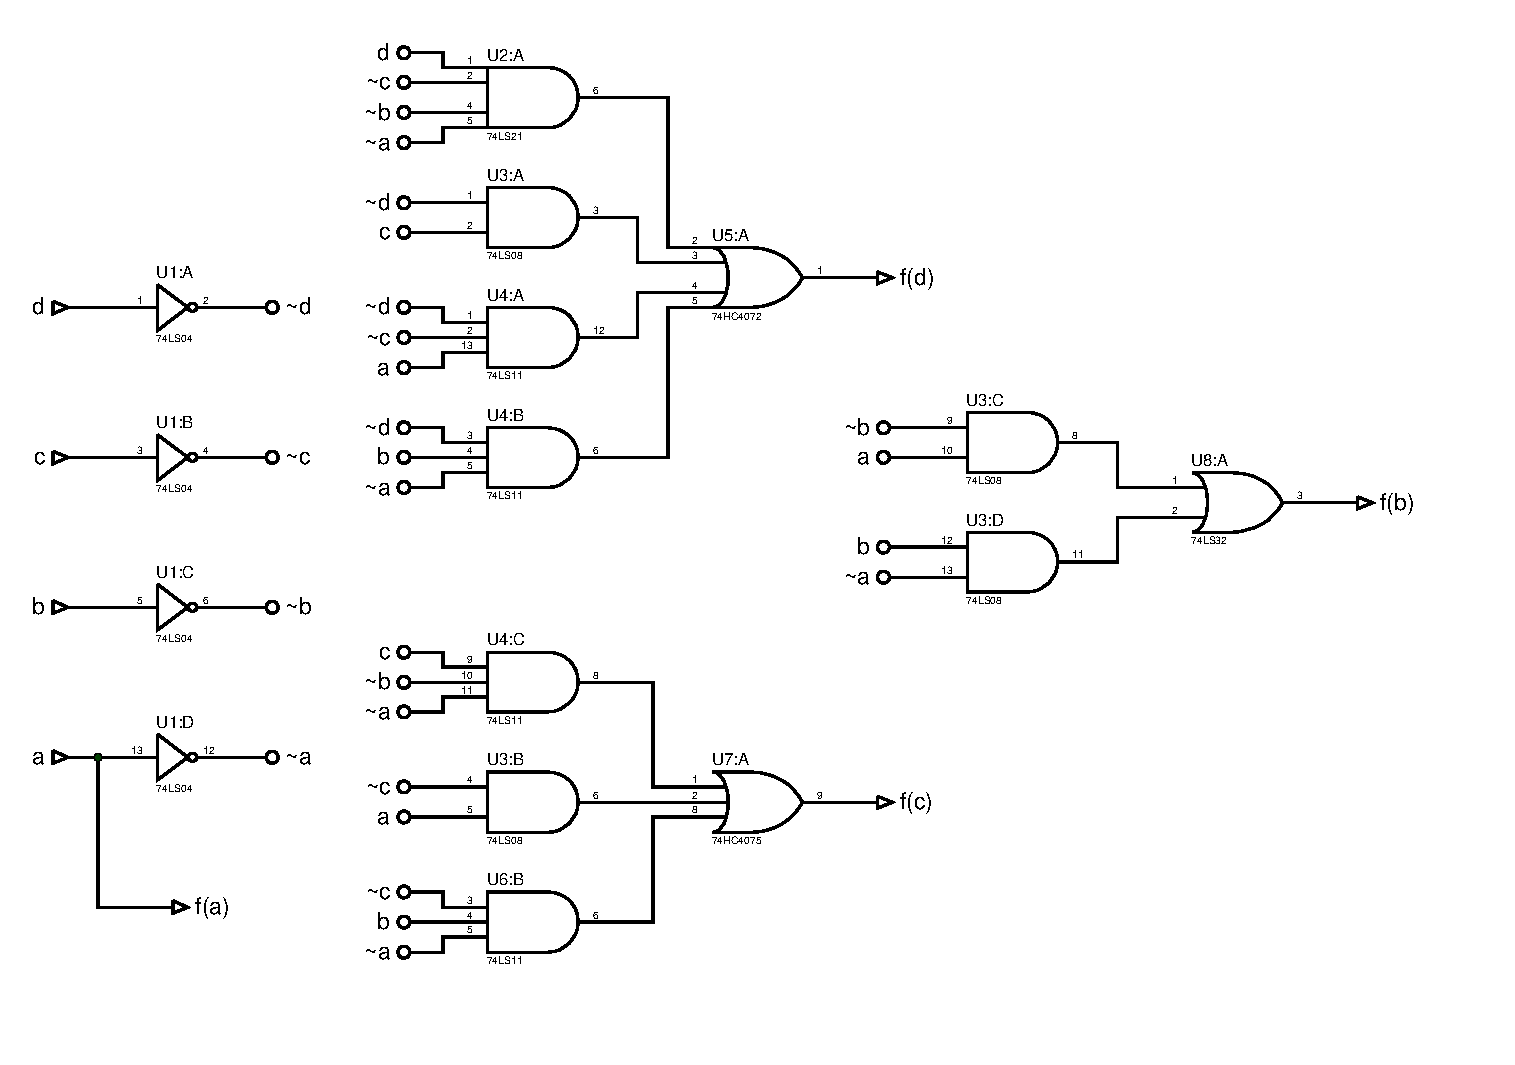
\includegraphics[width=1\textwidth]{data/ImplementacionEj4}
            \par\end{centering}
            \caption{data/Implementation of 2-complement circuit for a 4-bit input number - Designed in Proteus 7.8}
        \end{figure}
        
